% Options for packages loaded elsewhere
\PassOptionsToPackage{unicode}{hyperref}
\PassOptionsToPackage{hyphens}{url}
%
\documentclass[
  ignorenonframetext,
]{beamer}
\usepackage{pgfpages}
\setbeamertemplate{caption}[numbered]
\setbeamertemplate{caption label separator}{: }
\setbeamercolor{caption name}{fg=normal text.fg}
\beamertemplatenavigationsymbolsempty
% Prevent slide breaks in the middle of a paragraph
\widowpenalties 1 10000
\raggedbottom
\setbeamertemplate{part page}{
  \centering
  \begin{beamercolorbox}[sep=16pt,center]{part title}
    \usebeamerfont{part title}\insertpart\par
  \end{beamercolorbox}
}
\setbeamertemplate{section page}{
  \centering
  \begin{beamercolorbox}[sep=12pt,center]{part title}
    \usebeamerfont{section title}\insertsection\par
  \end{beamercolorbox}
}
\setbeamertemplate{subsection page}{
  \centering
  \begin{beamercolorbox}[sep=8pt,center]{part title}
    \usebeamerfont{subsection title}\insertsubsection\par
  \end{beamercolorbox}
}
\AtBeginPart{
  \frame{\partpage}
}
\AtBeginSection{
  \ifbibliography
  \else
    \frame{\sectionpage}
  \fi
}
\AtBeginSubsection{
  \frame{\subsectionpage}
}
\usepackage{amsmath,amssymb}
\usepackage{iftex}
\ifPDFTeX
  \usepackage[T1]{fontenc}
  \usepackage[utf8]{inputenc}
  \usepackage{textcomp} % provide euro and other symbols
\else % if luatex or xetex
  \usepackage{unicode-math} % this also loads fontspec
  \defaultfontfeatures{Scale=MatchLowercase}
  \defaultfontfeatures[\rmfamily]{Ligatures=TeX,Scale=1}
\fi
\usepackage{lmodern}
\usetheme[]{Warsaw}
\ifPDFTeX\else
  % xetex/luatex font selection
\fi
% Use upquote if available, for straight quotes in verbatim environments
\IfFileExists{upquote.sty}{\usepackage{upquote}}{}
\IfFileExists{microtype.sty}{% use microtype if available
  \usepackage[]{microtype}
  \UseMicrotypeSet[protrusion]{basicmath} % disable protrusion for tt fonts
}{}
\makeatletter
\@ifundefined{KOMAClassName}{% if non-KOMA class
  \IfFileExists{parskip.sty}{%
    \usepackage{parskip}
  }{% else
    \setlength{\parindent}{0pt}
    \setlength{\parskip}{6pt plus 2pt minus 1pt}}
}{% if KOMA class
  \KOMAoptions{parskip=half}}
\makeatother
\usepackage{xcolor}
\newif\ifbibliography
\usepackage{color}
\usepackage{fancyvrb}
\newcommand{\VerbBar}{|}
\newcommand{\VERB}{\Verb[commandchars=\\\{\}]}
\DefineVerbatimEnvironment{Highlighting}{Verbatim}{commandchars=\\\{\}}
% Add ',fontsize=\small' for more characters per line
\usepackage{framed}
\definecolor{shadecolor}{RGB}{248,248,248}
\newenvironment{Shaded}{\begin{snugshade}}{\end{snugshade}}
\newcommand{\AlertTok}[1]{\textcolor[rgb]{0.94,0.16,0.16}{#1}}
\newcommand{\AnnotationTok}[1]{\textcolor[rgb]{0.56,0.35,0.01}{\textbf{\textit{#1}}}}
\newcommand{\AttributeTok}[1]{\textcolor[rgb]{0.13,0.29,0.53}{#1}}
\newcommand{\BaseNTok}[1]{\textcolor[rgb]{0.00,0.00,0.81}{#1}}
\newcommand{\BuiltInTok}[1]{#1}
\newcommand{\CharTok}[1]{\textcolor[rgb]{0.31,0.60,0.02}{#1}}
\newcommand{\CommentTok}[1]{\textcolor[rgb]{0.56,0.35,0.01}{\textit{#1}}}
\newcommand{\CommentVarTok}[1]{\textcolor[rgb]{0.56,0.35,0.01}{\textbf{\textit{#1}}}}
\newcommand{\ConstantTok}[1]{\textcolor[rgb]{0.56,0.35,0.01}{#1}}
\newcommand{\ControlFlowTok}[1]{\textcolor[rgb]{0.13,0.29,0.53}{\textbf{#1}}}
\newcommand{\DataTypeTok}[1]{\textcolor[rgb]{0.13,0.29,0.53}{#1}}
\newcommand{\DecValTok}[1]{\textcolor[rgb]{0.00,0.00,0.81}{#1}}
\newcommand{\DocumentationTok}[1]{\textcolor[rgb]{0.56,0.35,0.01}{\textbf{\textit{#1}}}}
\newcommand{\ErrorTok}[1]{\textcolor[rgb]{0.64,0.00,0.00}{\textbf{#1}}}
\newcommand{\ExtensionTok}[1]{#1}
\newcommand{\FloatTok}[1]{\textcolor[rgb]{0.00,0.00,0.81}{#1}}
\newcommand{\FunctionTok}[1]{\textcolor[rgb]{0.13,0.29,0.53}{\textbf{#1}}}
\newcommand{\ImportTok}[1]{#1}
\newcommand{\InformationTok}[1]{\textcolor[rgb]{0.56,0.35,0.01}{\textbf{\textit{#1}}}}
\newcommand{\KeywordTok}[1]{\textcolor[rgb]{0.13,0.29,0.53}{\textbf{#1}}}
\newcommand{\NormalTok}[1]{#1}
\newcommand{\OperatorTok}[1]{\textcolor[rgb]{0.81,0.36,0.00}{\textbf{#1}}}
\newcommand{\OtherTok}[1]{\textcolor[rgb]{0.56,0.35,0.01}{#1}}
\newcommand{\PreprocessorTok}[1]{\textcolor[rgb]{0.56,0.35,0.01}{\textit{#1}}}
\newcommand{\RegionMarkerTok}[1]{#1}
\newcommand{\SpecialCharTok}[1]{\textcolor[rgb]{0.81,0.36,0.00}{\textbf{#1}}}
\newcommand{\SpecialStringTok}[1]{\textcolor[rgb]{0.31,0.60,0.02}{#1}}
\newcommand{\StringTok}[1]{\textcolor[rgb]{0.31,0.60,0.02}{#1}}
\newcommand{\VariableTok}[1]{\textcolor[rgb]{0.00,0.00,0.00}{#1}}
\newcommand{\VerbatimStringTok}[1]{\textcolor[rgb]{0.31,0.60,0.02}{#1}}
\newcommand{\WarningTok}[1]{\textcolor[rgb]{0.56,0.35,0.01}{\textbf{\textit{#1}}}}
\usepackage{longtable,booktabs,array}
\usepackage{calc} % for calculating minipage widths
\usepackage{caption}
% Make caption package work with longtable
\makeatletter
\def\fnum@table{\tablename~\thetable}
\makeatother
\usepackage{graphicx}
\makeatletter
\def\maxwidth{\ifdim\Gin@nat@width>\linewidth\linewidth\else\Gin@nat@width\fi}
\def\maxheight{\ifdim\Gin@nat@height>\textheight\textheight\else\Gin@nat@height\fi}
\makeatother
% Scale images if necessary, so that they will not overflow the page
% margins by default, and it is still possible to overwrite the defaults
% using explicit options in \includegraphics[width, height, ...]{}
\setkeys{Gin}{width=\maxwidth,height=\maxheight,keepaspectratio}
% Set default figure placement to htbp
\makeatletter
\def\fps@figure{htbp}
\makeatother
\setlength{\emergencystretch}{3em} % prevent overfull lines
\providecommand{\tightlist}{%
  \setlength{\itemsep}{0pt}\setlength{\parskip}{0pt}}
\setcounter{secnumdepth}{-\maxdimen} % remove section numbering
\usepackage{amsmath}
\ifLuaTeX
  \usepackage{selnolig}  % disable illegal ligatures
\fi
\IfFileExists{bookmark.sty}{\usepackage{bookmark}}{\usepackage{hyperref}}
\IfFileExists{xurl.sty}{\usepackage{xurl}}{} % add URL line breaks if available
\urlstyle{same}
\hypersetup{
  pdftitle={Building Shiny Apps},
  hidelinks,
  pdfcreator={LaTeX via pandoc}}

\title{Building Shiny Apps}
\author{W. Evan Johnson, Ph.D.\\
Professor, Division of Infectious Disease\\
Director, Center for Data Science\\
Rutgers University -- New Jersey Medical School}
\date{11/17/2023}

\begin{document}
\frame{\titlepage}

\begin{frame}[fragile]{What is Shiny?}
\phantomsection\label{what-is-shiny}
\texttt{Shiny} is an R package that allows you to easily create rich,
interactive web apps around your R functions and packages.
\texttt{Shiny} allows you to take your work in R and disseminate it via
a web browser so that anyone can use it. \texttt{Shiny} makes you look
awesome by making it easy to produce polished web apps with a minimum
amount of pain.

(Credit: Some of the images and slide text were taken and adapted from
\url{https://mastering-shiny.org} and RStudio's \texttt{Shiny}
tutorials)
\end{frame}

\begin{frame}[fragile]{What is Shiny?}
\phantomsection\label{what-is-shiny-1}
\texttt{Shiny} is designed primarily with data scientists in mind, and
to that end, you can create pretty complicated \texttt{Shiny} apps with
no knowledge of HTML, CSS, or JavaScript. On the other hand,
\texttt{Shiny} doesn't limit you to creating trivial or prefabricated
apps: its user interface components can be easily customized or
extended, and its server uses reactive programming to let you create any
type of back end logic you want.
\end{frame}

\begin{frame}[fragile]{What is Shiny?}
\phantomsection\label{what-is-shiny-2}
Some of the things people use \texttt{Shiny} for are:

\begin{itemize}
\tightlist
\item
  Create dashboards
\item
  Replace hundreds of pages of PDFs with interactive apps
\item
  Communicate complex models informative visualizations
\item
  Provide self-service data analysis for common workflows
\item
  Create interactive demos for teaching statistics and data science
\end{itemize}

In short, \texttt{Shiny} gives you the ability to pass on some of your
\texttt{R} superpowers to anyone who can use the web.
\end{frame}

\begin{frame}[fragile]{Getting Started}
\phantomsection\label{getting-started}
To create your first \texttt{Shiny} App you wil need:

\begin{itemize}
\tightlist
\item
  Install R: Come on now!!
\item
  Install RStudio (strongly recommended):
  \url{https://www.rstudio.com/products/rstudio/download}
\item
  The R \texttt{Shiny} package: \texttt{install.packages("shiny")}
\item
  Knowledge and experience in developing R packages (recommended)
\item
  Git and GitHub (recommended): to share your Apps
\end{itemize}
\end{frame}

\begin{frame}[fragile]{Getting Started}
\phantomsection\label{getting-started-1}
If you haven't already installed \texttt{Shiny}, install it now with:

\begin{Shaded}
\begin{Highlighting}[]
\FunctionTok{install.packages}\NormalTok{(}\StringTok{"shiny"}\NormalTok{)}
\end{Highlighting}
\end{Shaded}

If you've already installed \texttt{Shiny}, use the following to check
that you have version 1.5.0 or greater:

\begin{Shaded}
\begin{Highlighting}[]
\FunctionTok{packageVersion}\NormalTok{(}\StringTok{"shiny"}\NormalTok{) }
\end{Highlighting}
\end{Shaded}

\begin{verbatim}
## [1] '1.7.5.1'
\end{verbatim}
\end{frame}

\begin{frame}[fragile]{Shiny Introduction}
\phantomsection\label{shiny-introduction}
RStudio's
\href{www.rstudio.com/products/shiny/shiny-user-showcase/}{Shiny
Showcase} is an exciting assembly of exciting apps!

Or we can start with a very simple example

\begin{Shaded}
\begin{Highlighting}[]
\FunctionTok{library}\NormalTok{(shiny)}
\FunctionTok{runExample}\NormalTok{(}\StringTok{"01\_hello"}\NormalTok{)}
\end{Highlighting}
\end{Shaded}
\end{frame}

\begin{frame}[fragile]{Shiny Introduction}
\phantomsection\label{shiny-introduction-1}
Or an example from Dr.~Johnson's research:

\begin{Shaded}
\begin{Highlighting}[]
\NormalTok{devtools}\SpecialCharTok{::}\FunctionTok{install\_github}\NormalTok{(}\StringTok{"compbiomed/animalcules"}\NormalTok{)}
\FunctionTok{library}\NormalTok{(animalcules)}
\FunctionTok{run\_animalcules}\NormalTok{()}
\end{Highlighting}
\end{Shaded}

(Warning: this might take a while to load package dependencies!)
\end{frame}

\begin{frame}{Shiny Architecture}
\phantomsection\label{shiny-architecture}
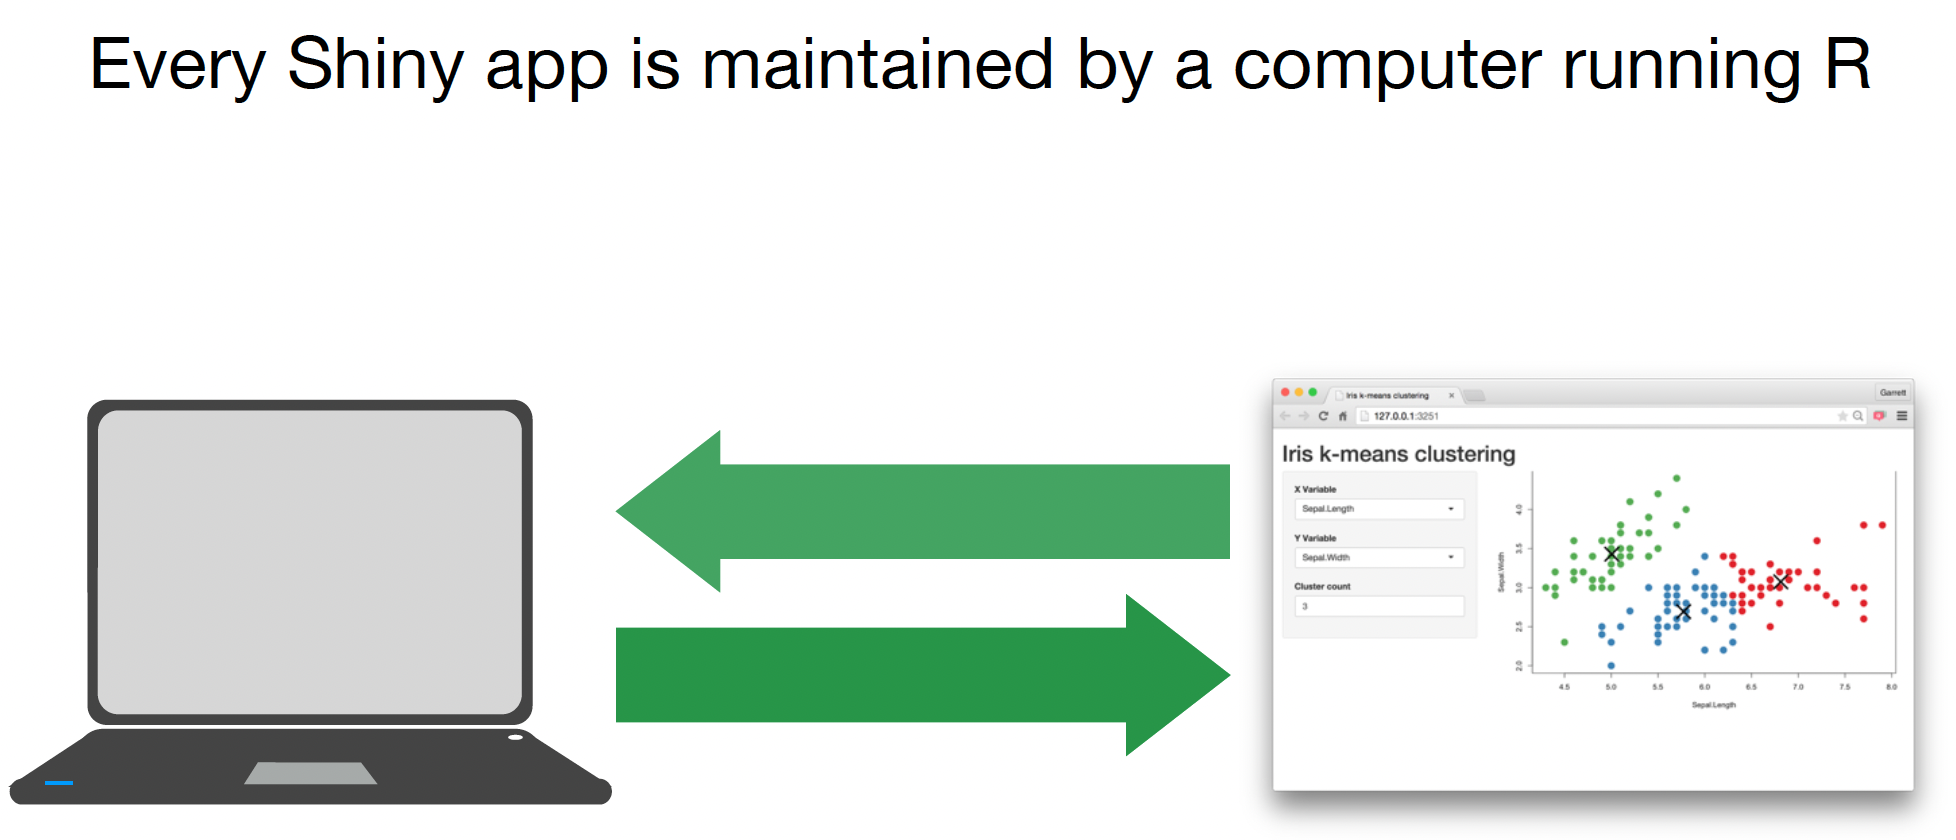
\includegraphics{shinyfigs/shiny_arch_1.png}
\end{frame}

\begin{frame}{Shiny Architecture}
\phantomsection\label{shiny-architecture-1}
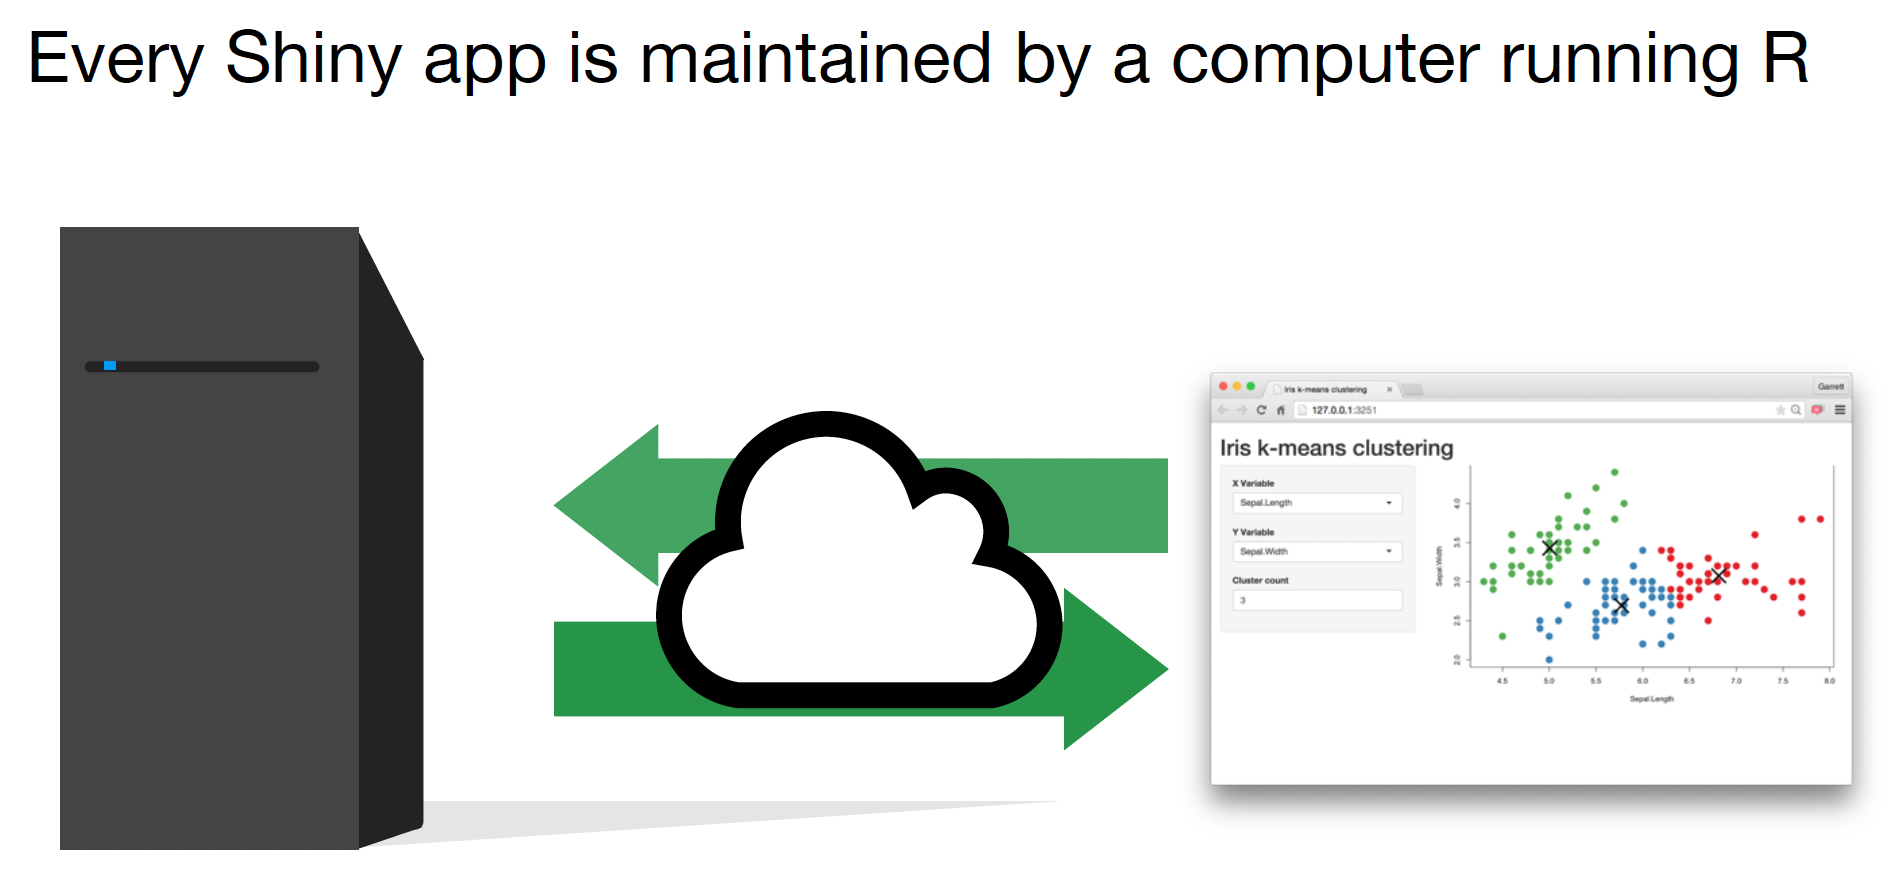
\includegraphics{shinyfigs/shiny_arch_2.png}
\end{frame}

\begin{frame}{Shiny Architecture}
\phantomsection\label{shiny-architecture-2}
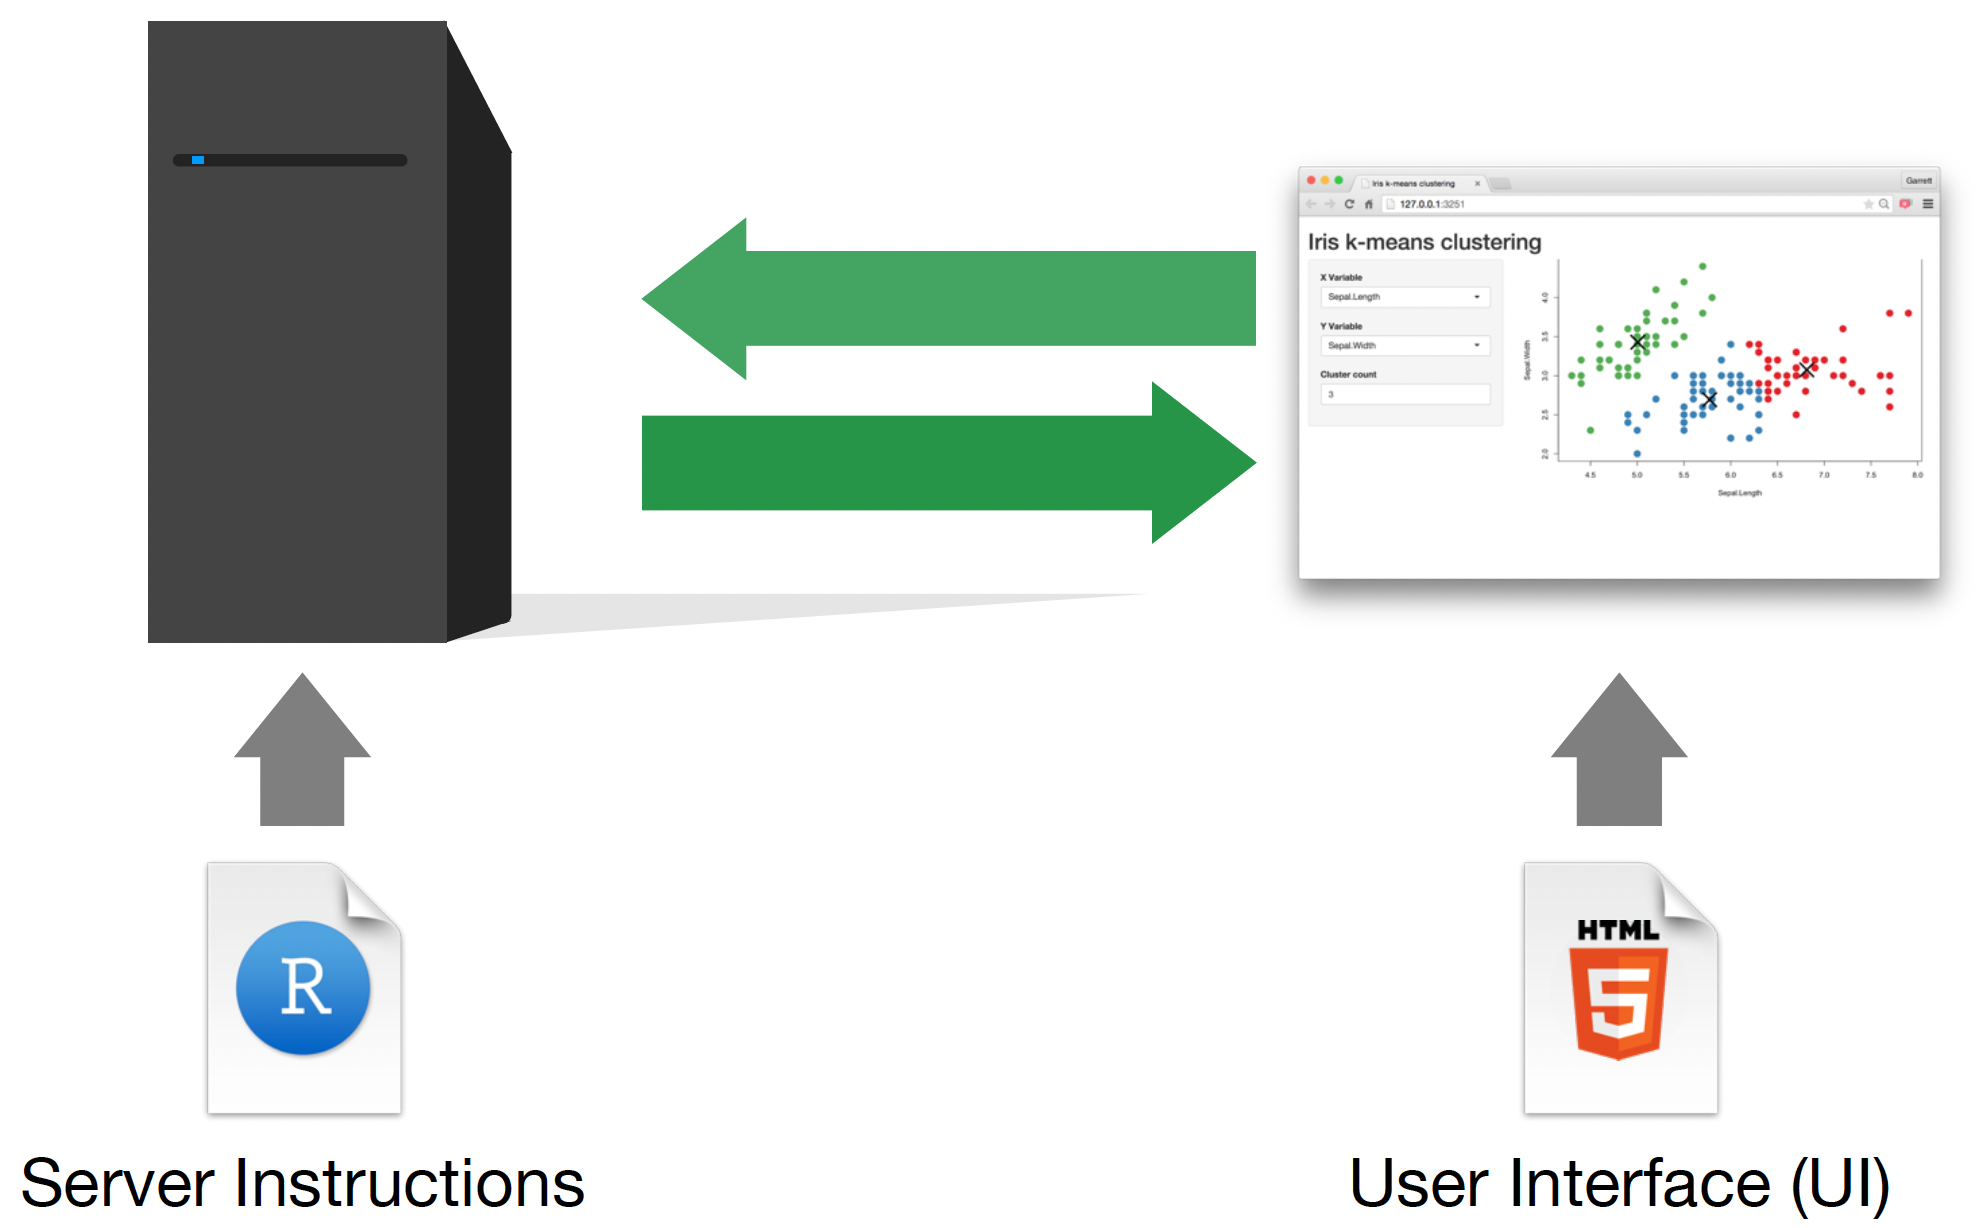
\includegraphics{shinyfigs/shiny_arch_3.png}
\end{frame}

\begin{frame}[fragile]{Introduction to shiny development}
\phantomsection\label{introduction-to-shiny-development}
Here we'll create a simple \texttt{Shiny} app, staring with the minimum
boilerplate, followed by the two key components of every \texttt{Shiny}
app: the UI (short for user interface) which defines how your app looks,
and the server function which defines how your app works. \texttt{Shiny}
uses \textbf{reactive} programming to automatically update outputs when
inputs change.
\end{frame}

\begin{frame}[fragile]{Template: shortest viable app}
\phantomsection\label{template-shortest-viable-app}
The simplest way to start an app is to create a new directory, and add a
single file called app.R, with the following code:

\begin{Shaded}
\begin{Highlighting}[]
\FunctionTok{library}\NormalTok{(shiny)}

\NormalTok{ui }\OtherTok{\textless{}{-}} \FunctionTok{fluidPage}\NormalTok{()}

\NormalTok{server }\OtherTok{\textless{}{-}} \ControlFlowTok{function}\NormalTok{(input, output) \{\}}

\FunctionTok{shinyApp}\NormalTok{(}\AttributeTok{ui =}\NormalTok{ ui, }\AttributeTok{server =}\NormalTok{ server)}
\end{Highlighting}
\end{Shaded}
\end{frame}

\begin{frame}{Close your app}
\phantomsection\label{close-your-app}
\center

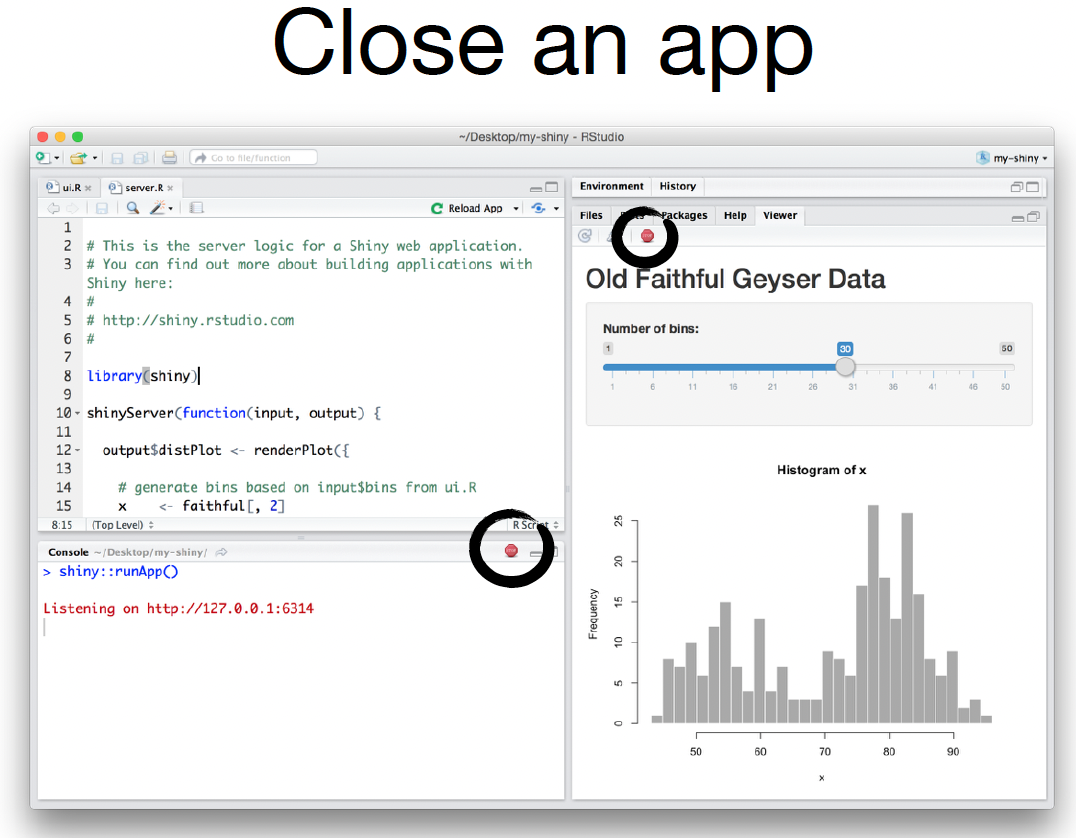
\includegraphics{shinyfigs/shiny_off.png}
\end{frame}

\begin{frame}{Inputs and outputs}
\phantomsection\label{inputs-and-outputs}
\center

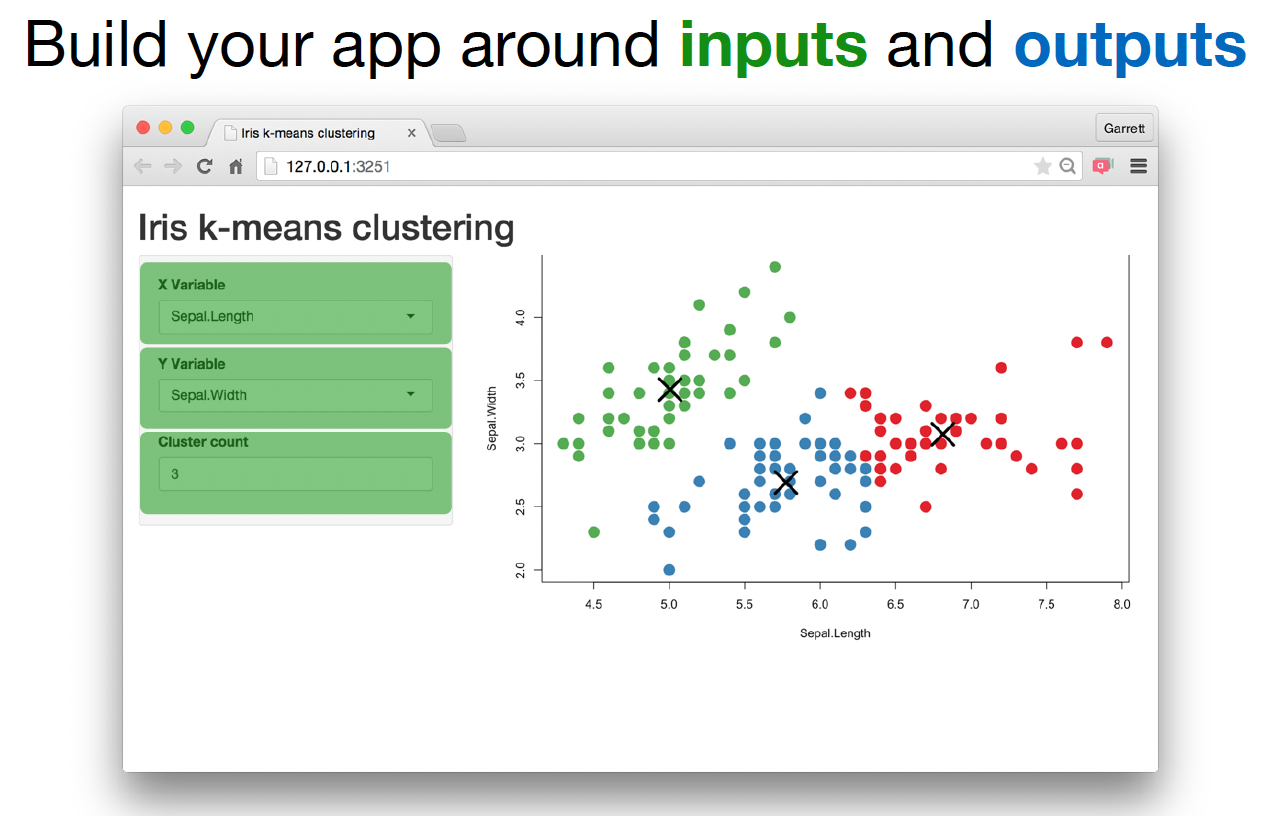
\includegraphics{shinyfigs/shiny_in_out.png}
\end{frame}

\begin{frame}{Inputs and outputs}
\phantomsection\label{inputs-and-outputs-1}
\center

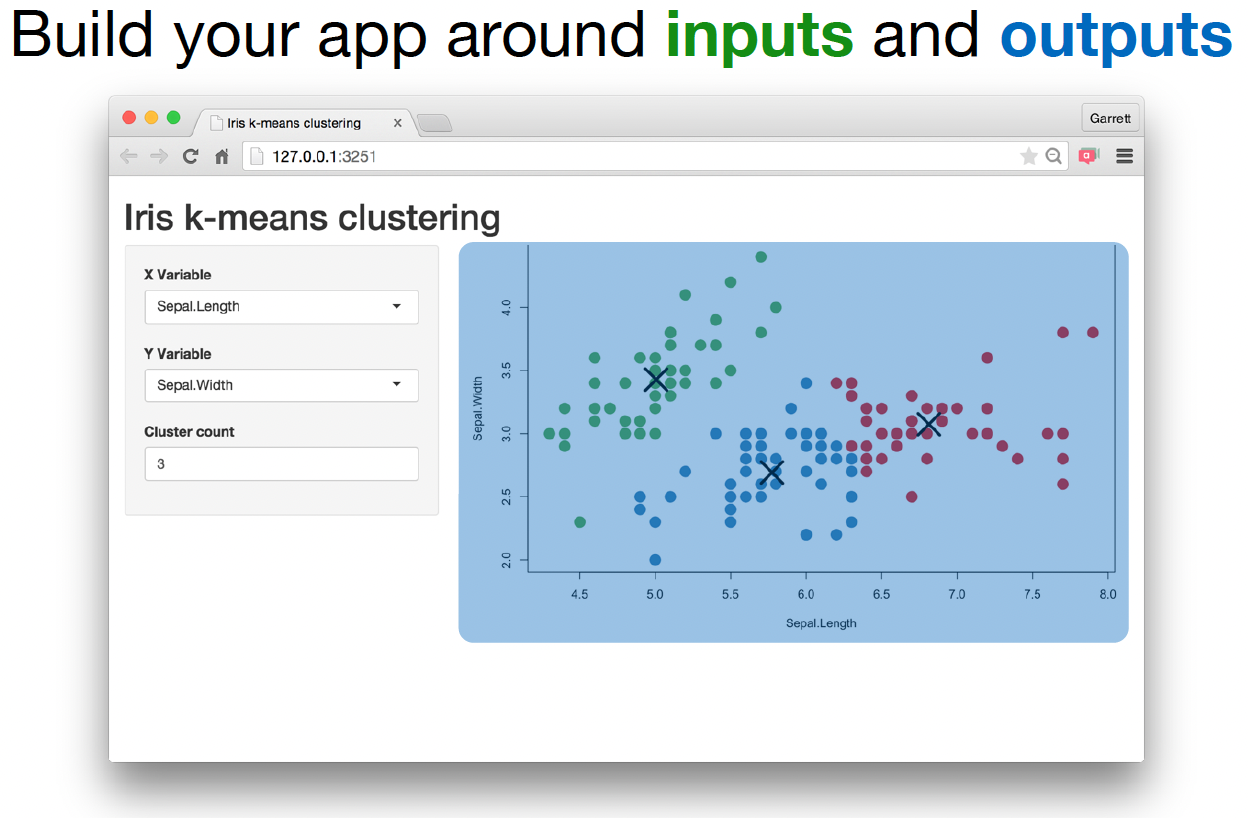
\includegraphics{shinyfigs/shiny_in_out_1.png}
\end{frame}

\begin{frame}[fragile]{Adding elements to the UI}
\phantomsection\label{adding-elements-to-the-ui}
Add elements to your app as arguments to fluidPage()

\begin{Shaded}
\begin{Highlighting}[]
\FunctionTok{library}\NormalTok{(shiny)}

\NormalTok{ui }\OtherTok{\textless{}{-}} \FunctionTok{fluidPage}\NormalTok{(}
    \CommentTok{\# Input() functions,}
    \CommentTok{\# Output() functions}
\NormalTok{    )}

\NormalTok{server }\OtherTok{\textless{}{-}} \ControlFlowTok{function}\NormalTok{(input, output) \{\}}

\FunctionTok{shinyApp}\NormalTok{(}\AttributeTok{ui =}\NormalTok{ ui, }\AttributeTok{server =}\NormalTok{ server)}
\end{Highlighting}
\end{Shaded}
\end{frame}

\begin{frame}[fragile]{Adding elements to the UI}
\phantomsection\label{adding-elements-to-the-ui-1}
Add elements to your app as arguments to \texttt{fluidPage()}

\begin{Shaded}
\begin{Highlighting}[]
\FunctionTok{library}\NormalTok{(shiny)}

\NormalTok{ui }\OtherTok{\textless{}{-}} \FunctionTok{fluidPage}\NormalTok{(}
  \StringTok{"Hello World!"}
\NormalTok{  )}

\NormalTok{server }\OtherTok{\textless{}{-}} \ControlFlowTok{function}\NormalTok{(input, output) \{\}}

\FunctionTok{shinyApp}\NormalTok{(}\AttributeTok{ui =}\NormalTok{ ui, }\AttributeTok{server =}\NormalTok{ server)}
\end{Highlighting}
\end{Shaded}
\end{frame}

\begin{frame}[fragile]{Input functions}
\phantomsection\label{input-functions}
Create an input with an \textbf{Input()} function.

\begin{Shaded}
\begin{Highlighting}[]
\FunctionTok{sliderInput}\NormalTok{(}\AttributeTok{inputId =} \StringTok{"num"}\NormalTok{, }
            \AttributeTok{label =} \StringTok{"Choose a number"}\NormalTok{, }
            \AttributeTok{value =} \DecValTok{25}\NormalTok{, }\AttributeTok{min =} \DecValTok{1}\NormalTok{, }\AttributeTok{max =} \DecValTok{100}\NormalTok{)}
\end{Highlighting}
\end{Shaded}

Here is the actual HTML code for this slider: \footnotesize

\begin{Shaded}
\begin{Highlighting}[]
\DataTypeTok{\textless{}}\KeywordTok{div}\OtherTok{ class}\OperatorTok{=}\StringTok{"form{-}group shiny{-}input{-}container"}\DataTypeTok{\textgreater{}}
  \DataTypeTok{\textless{}}\KeywordTok{label}\OtherTok{ class}\OperatorTok{=}\StringTok{"control{-}label"}\OtherTok{ for}\OperatorTok{=}\StringTok{"num"}\DataTypeTok{\textgreater{}}\NormalTok{Choose a number}\DataTypeTok{\textless{}/}\KeywordTok{label}\DataTypeTok{\textgreater{}}
  \DataTypeTok{\textless{}}\KeywordTok{input}\OtherTok{ class}\OperatorTok{=}\StringTok{"js{-}range{-}slider"}\OtherTok{ id}\OperatorTok{=}\StringTok{"num"}\OtherTok{ data{-}min}\OperatorTok{=}\StringTok{"1"}\OtherTok{ data{-}max}\OperatorTok{=}\StringTok{"100"}
\OtherTok{  data{-}from}\OperatorTok{=}\StringTok{"25"}\OtherTok{ data{-}step}\OperatorTok{=}\StringTok{"1"}\OtherTok{ data{-}grid}\OperatorTok{=}\StringTok{"true"}\OtherTok{ data{-}grid{-}num}\OperatorTok{=}\StringTok{"9.9"}
\OtherTok{  data{-}grid{-}snap}\OperatorTok{=}\StringTok{"false"}\OtherTok{ data{-}prettify{-}separator}\OperatorTok{=}\StringTok{","}\OtherTok{ data{-}keyboard}\OperatorTok{=}\StringTok{"true"}
\OtherTok{  data{-}keyboard{-}step}\OperatorTok{=}\StringTok{"1.01010101010101"}\DataTypeTok{/\textgreater{}}
\DataTypeTok{\textless{}/}\KeywordTok{div}\DataTypeTok{\textgreater{}}
\end{Highlighting}
\end{Shaded}
\end{frame}

\begin{frame}{Shiny buttons}
\phantomsection\label{shiny-buttons}
\center

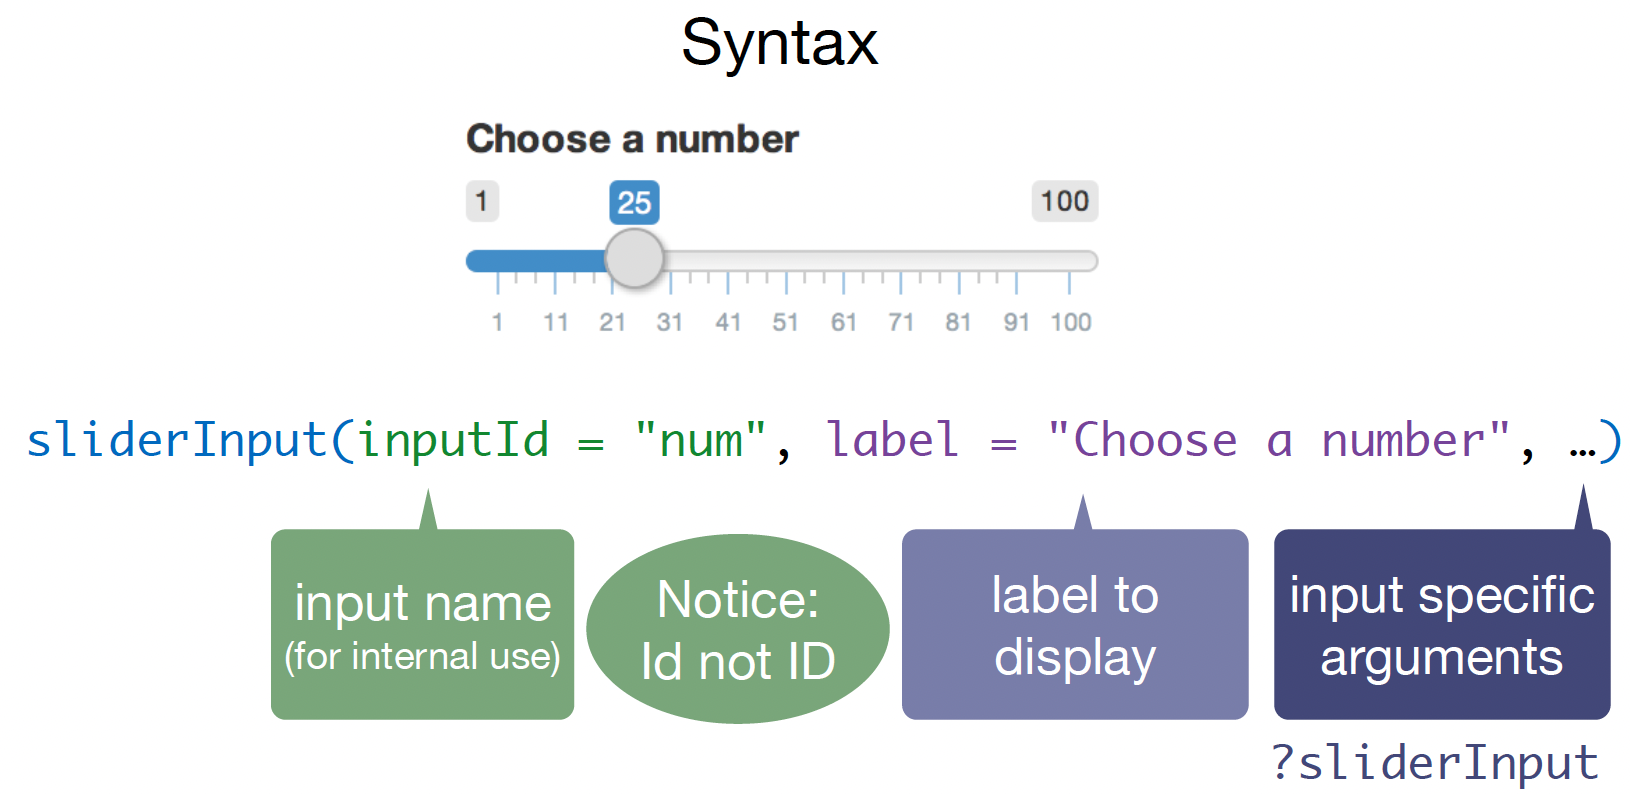
\includegraphics{shinyfigs/shiny_buttons_syntax.png}
\end{frame}

\begin{frame}[fragile]{Input functions in an app}
\phantomsection\label{input-functions-in-an-app}
Create an input with an \textbf{Input()} function.

\begin{Shaded}
\begin{Highlighting}[]
\FunctionTok{library}\NormalTok{(shiny)}

\NormalTok{ui }\OtherTok{\textless{}{-}} \FunctionTok{fluidPage}\NormalTok{(}
  \FunctionTok{sliderInput}\NormalTok{(}\AttributeTok{inputId =} \StringTok{"num"}\NormalTok{,}
    \AttributeTok{label =} \StringTok{"Choose a number"}\NormalTok{,}
    \AttributeTok{value =} \DecValTok{25}\NormalTok{, }\AttributeTok{min =} \DecValTok{1}\NormalTok{, }\AttributeTok{max =} \DecValTok{100}\NormalTok{)}
\NormalTok{  )}

\NormalTok{server }\OtherTok{\textless{}{-}} \ControlFlowTok{function}\NormalTok{(input, output) \{\}}

\FunctionTok{shinyApp}\NormalTok{(}\AttributeTok{server =}\NormalTok{ server, }\AttributeTok{ui =}\NormalTok{ ui)}
\end{Highlighting}
\end{Shaded}
\end{frame}

\begin{frame}{Shiny buttons}
\phantomsection\label{shiny-buttons-1}
\center

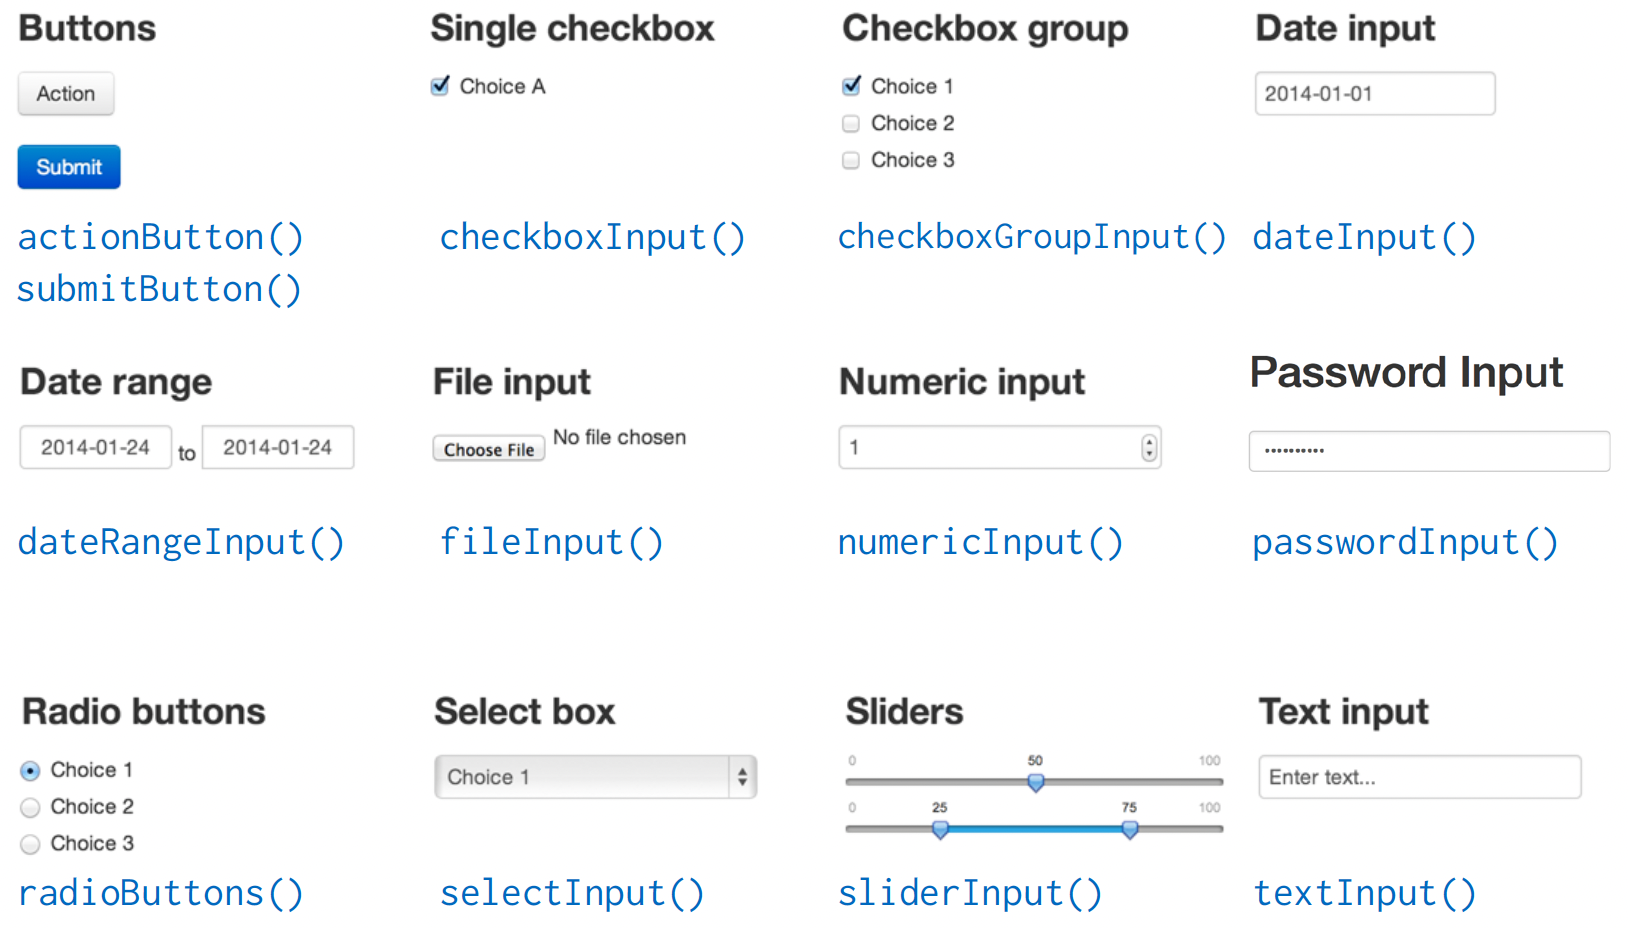
\includegraphics{shinyfigs/shiny_buttons.png}
\end{frame}

\begin{frame}{Shiny outputs}
\phantomsection\label{shiny-outputs}
\center

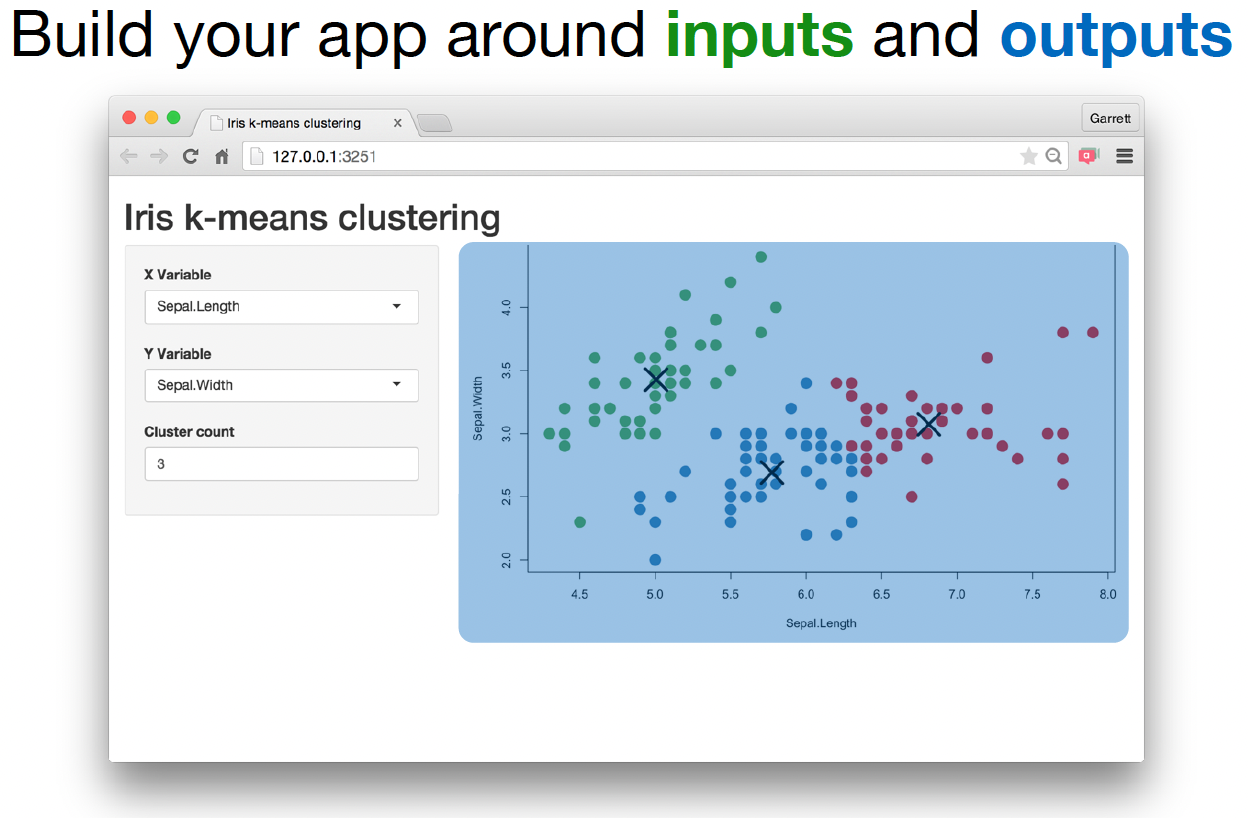
\includegraphics{shinyfigs/shiny_in_out_1.png} \#\# Shiny outputs
\center 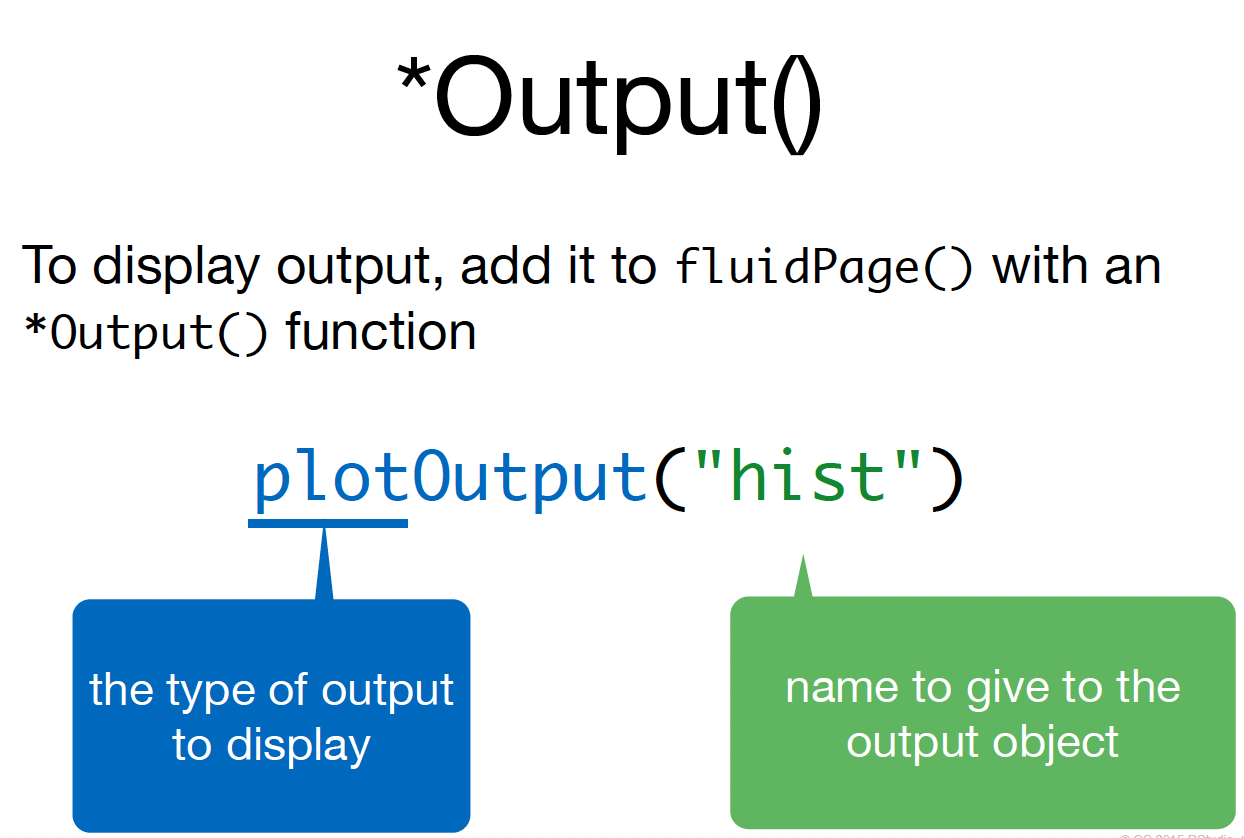
\includegraphics{shinyfigs/shiny_output1.png}
\end{frame}

\begin{frame}{Shiny outputs}
\phantomsection\label{shiny-outputs-1}
\center

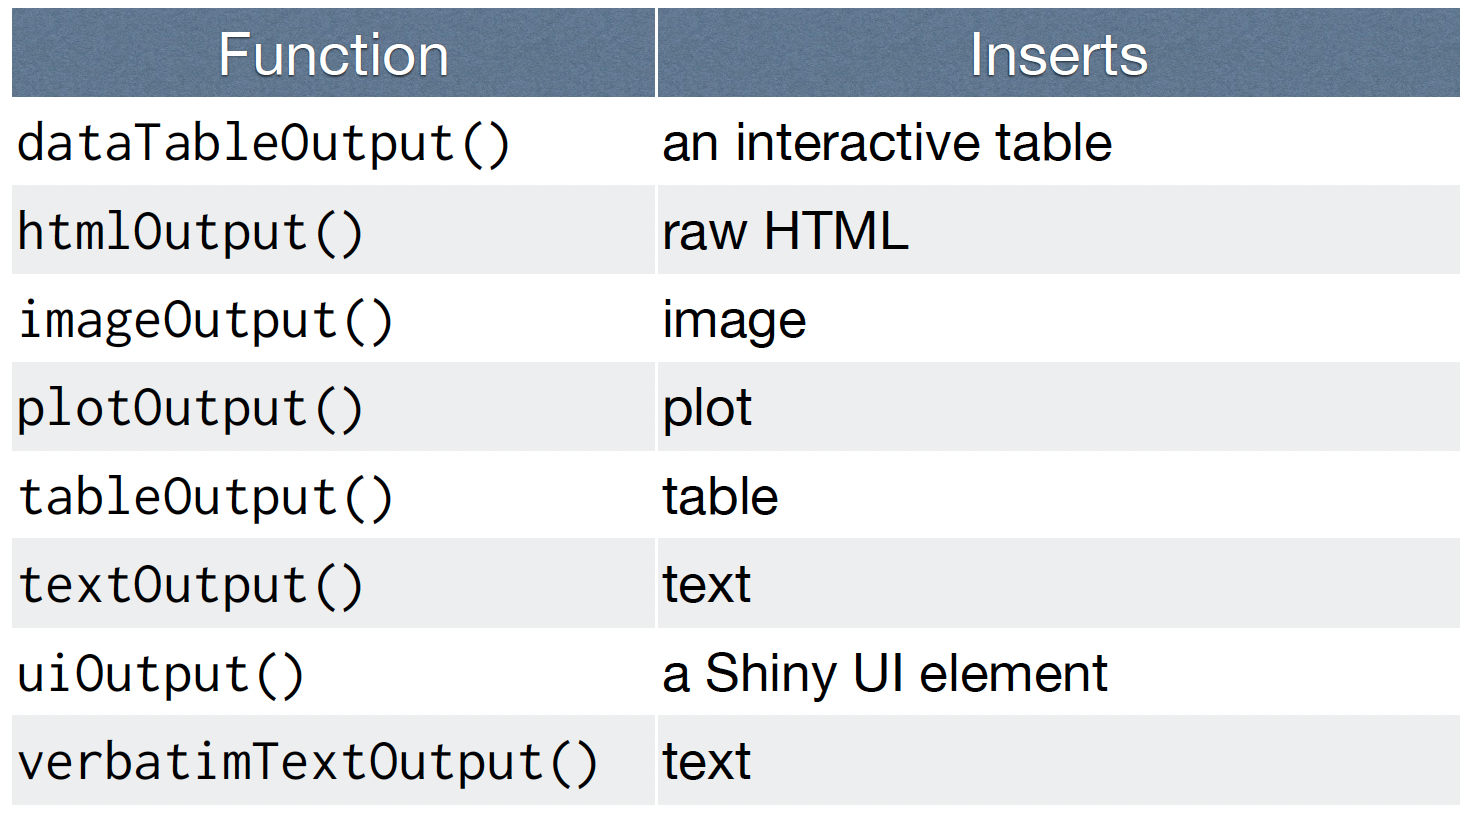
\includegraphics{shinyfigs/shiny_output2.png}
\end{frame}

\begin{frame}[fragile]{Adding outputs}
\phantomsection\label{adding-outputs}
Create an output with an \textbf{Output()} function.

\begin{Shaded}
\begin{Highlighting}[]
\FunctionTok{library}\NormalTok{(shiny)}

\NormalTok{ui }\OtherTok{\textless{}{-}} \FunctionTok{fluidPage}\NormalTok{(}
  \FunctionTok{sliderInput}\NormalTok{(}\AttributeTok{inputId =} \StringTok{"num"}\NormalTok{,}
    \AttributeTok{label =} \StringTok{"Choose a number"}\NormalTok{,}
    \AttributeTok{value =} \DecValTok{25}\NormalTok{, }\AttributeTok{min =} \DecValTok{1}\NormalTok{, }\AttributeTok{max =} \DecValTok{100}\NormalTok{), }\DocumentationTok{\#\# Note the comma!}
  \FunctionTok{plotOutput}\NormalTok{(}\StringTok{"hist"}\NormalTok{)}
\NormalTok{  )}

\NormalTok{server }\OtherTok{\textless{}{-}} \ControlFlowTok{function}\NormalTok{(input, output) \{\}}

\FunctionTok{shinyApp}\NormalTok{(}\AttributeTok{server =}\NormalTok{ server, }\AttributeTok{ui =}\NormalTok{ ui)}
\end{Highlighting}
\end{Shaded}

Note that you must build the output in the server first!
\end{frame}

\begin{frame}{Shiny outputs}
\phantomsection\label{shiny-outputs-2}
\center

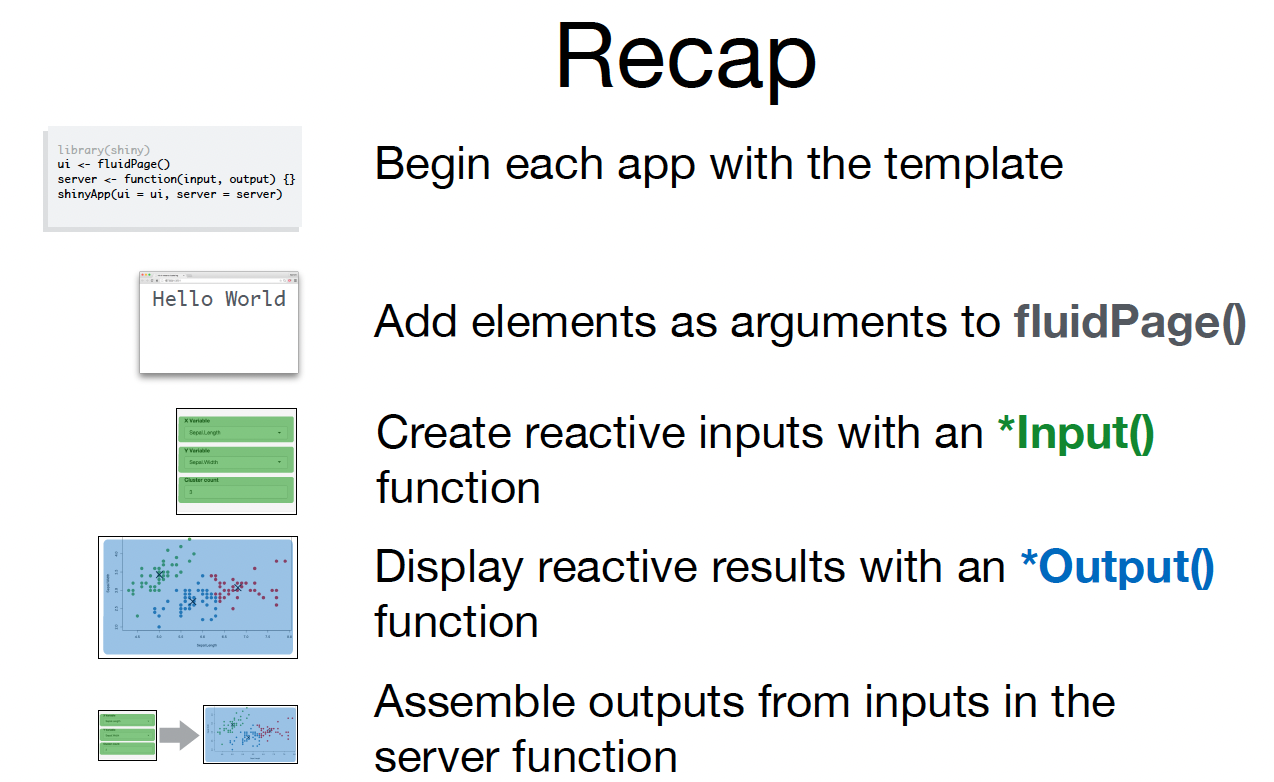
\includegraphics{shinyfigs/shiny_recap1.png}
\end{frame}

\begin{frame}{Building the server}
\phantomsection\label{building-the-server}
There are 3 basic rules for your \textbf{server} function:

\begin{enumerate}
\tightlist
\item
  Access input values with \textbf{input\$}
\item
  Save objects to display as \textbf{output\$}
\item
  Build objects to display with \textbf{render()}
\end{enumerate}
\end{frame}

\begin{frame}{Server inputs}
\phantomsection\label{server-inputs}
You can access inputs from the UI using \textbf{input\$} \center
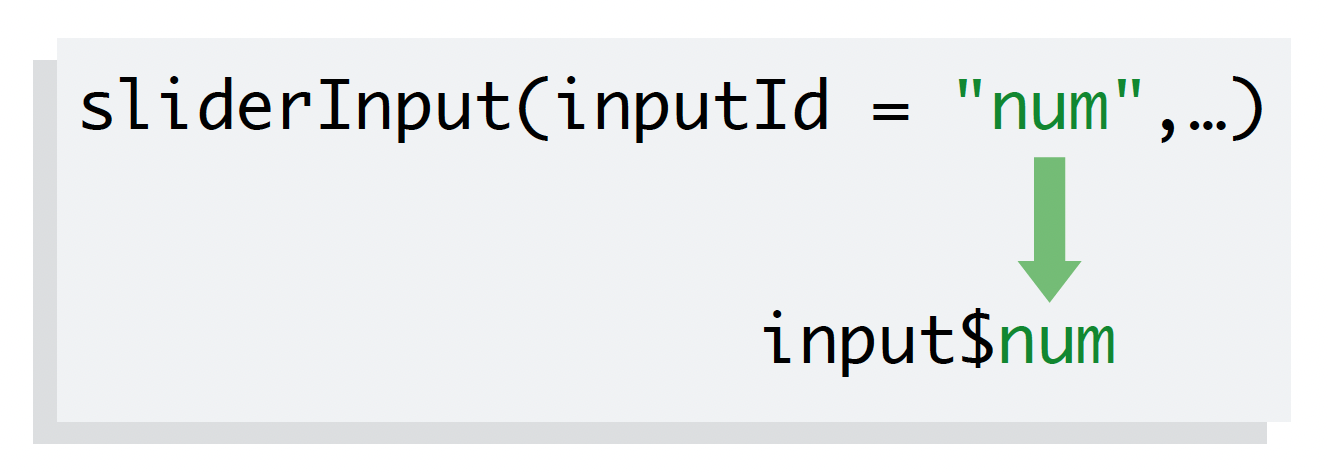
\includegraphics{shinyfigs/shiny_server_inputs1.png}
\end{frame}

\begin{frame}{}
\phantomsection\label{section}
\center

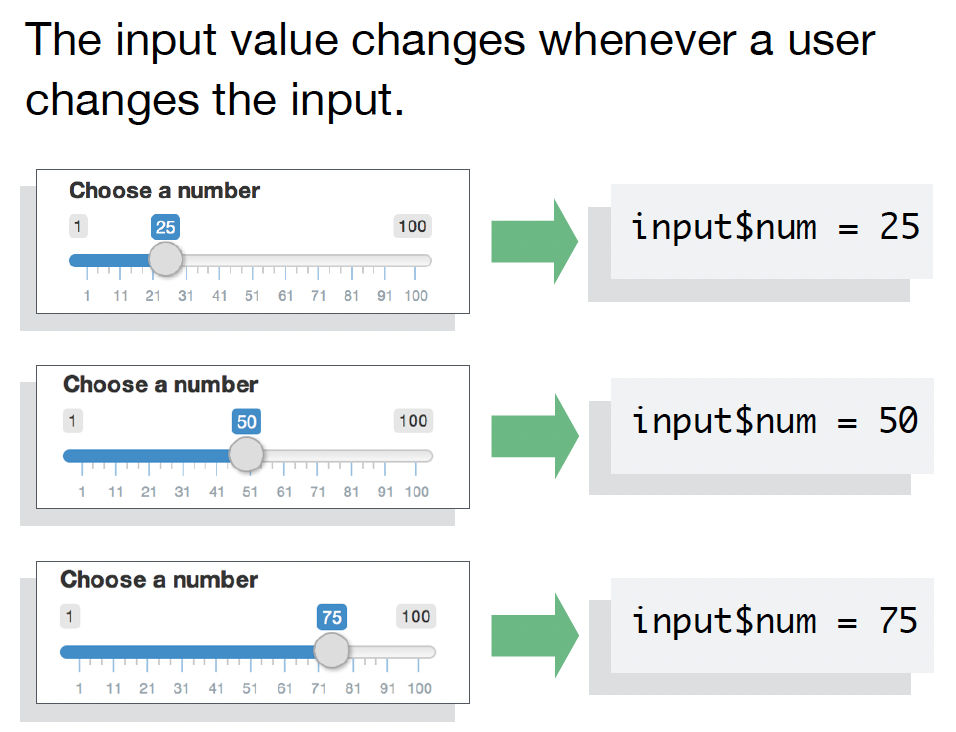
\includegraphics{shinyfigs/shiny_server_inputs2.png} \#\# Server outputs
You can save your outputs to return to the UI using \textbf{output\$}
\center 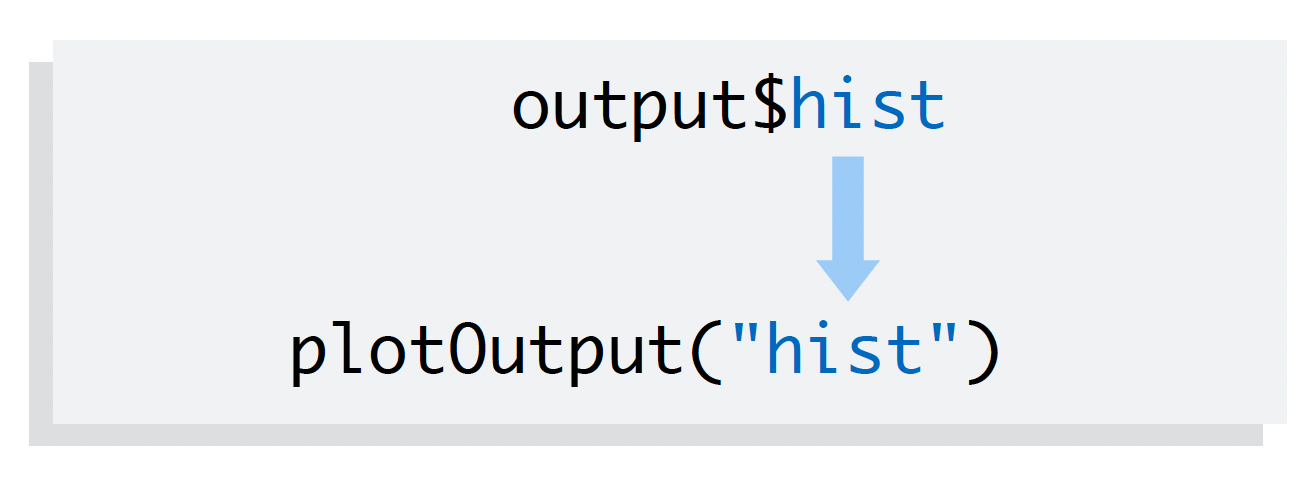
\includegraphics{shinyfigs/shiny_server_output1.png}
\end{frame}

\begin{frame}{Server outputs}
\phantomsection\label{server-outputs}
You can save your outputs to return to the UI using \textbf{output\$}
\center 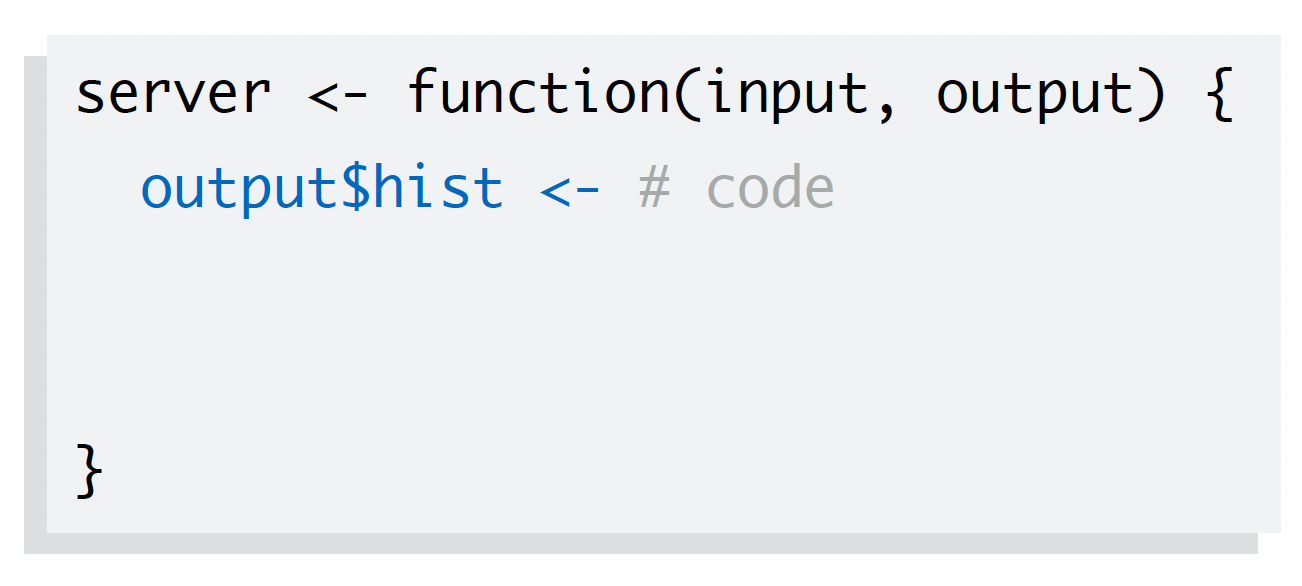
\includegraphics{shinyfigs/shiny_server_output2.png}
\end{frame}

\begin{frame}{Rendering server outputs}
\phantomsection\label{rendering-server-outputs}
Build objects to display with \textbf{render()} \center
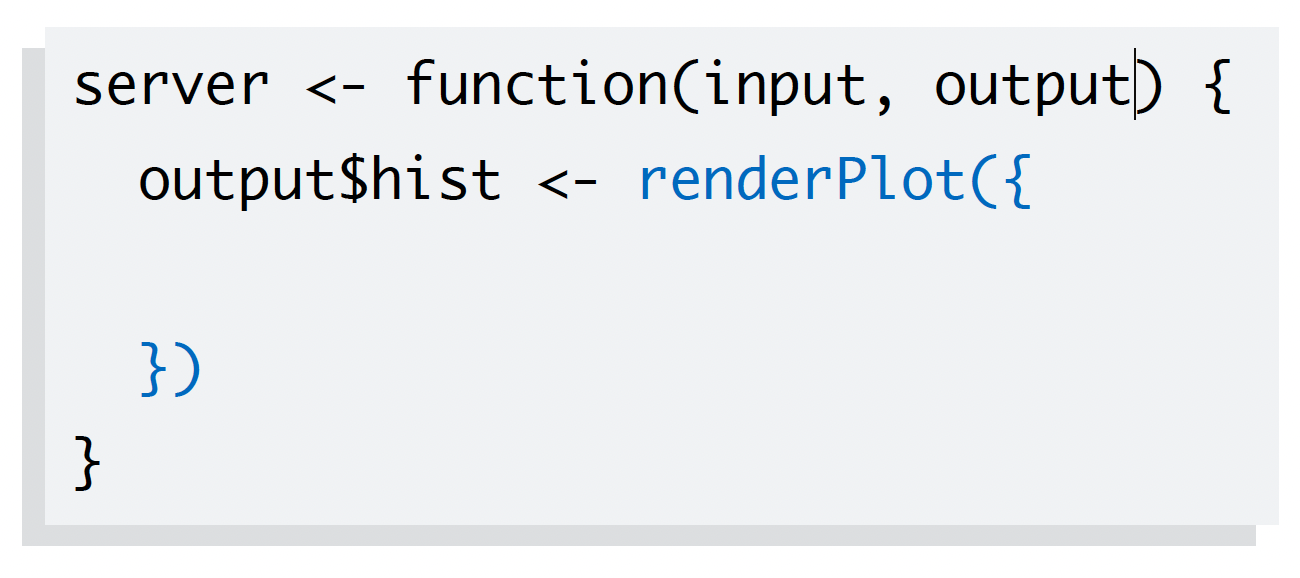
\includegraphics{shinyfigs/shiny_render1.png}
\end{frame}

\begin{frame}{Rendering server outputs}
\phantomsection\label{rendering-server-outputs-1}
\center

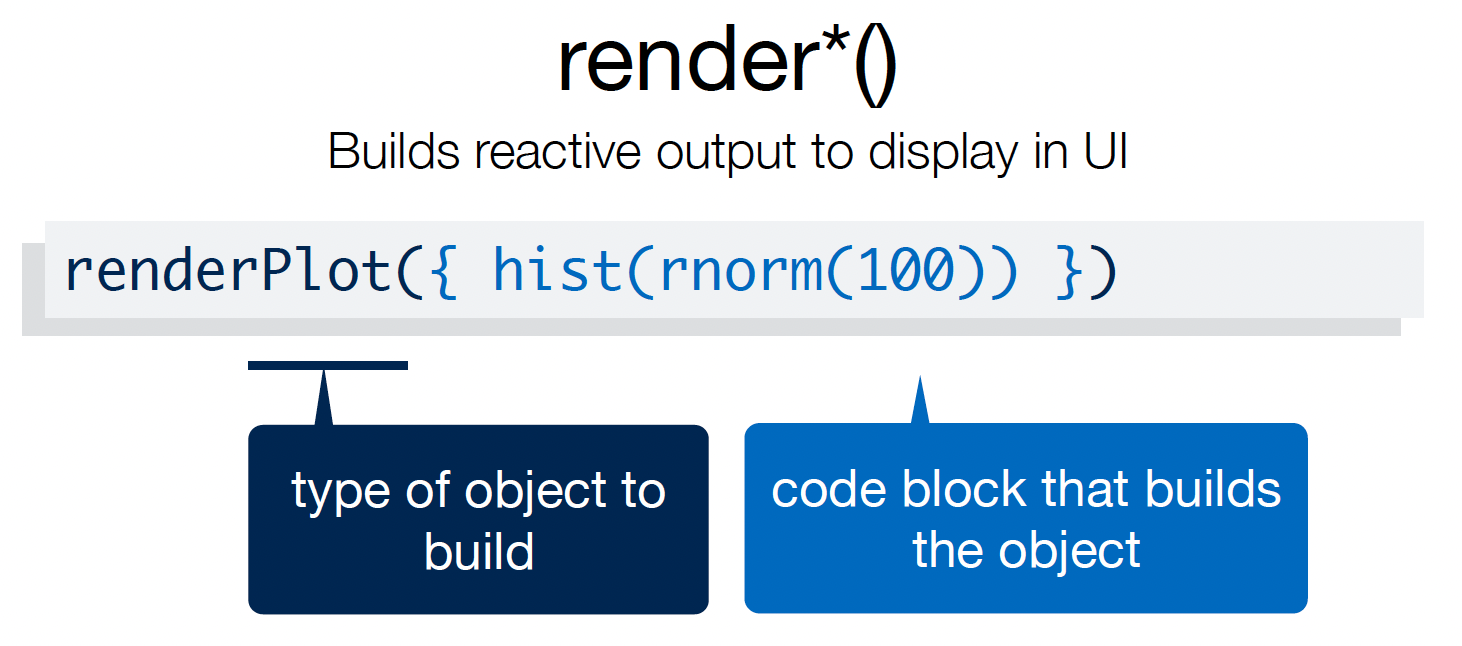
\includegraphics{shinyfigs/shiny_render2.png}
\end{frame}

\begin{frame}{Rendering server outputs}
\phantomsection\label{rendering-server-outputs-2}
\center

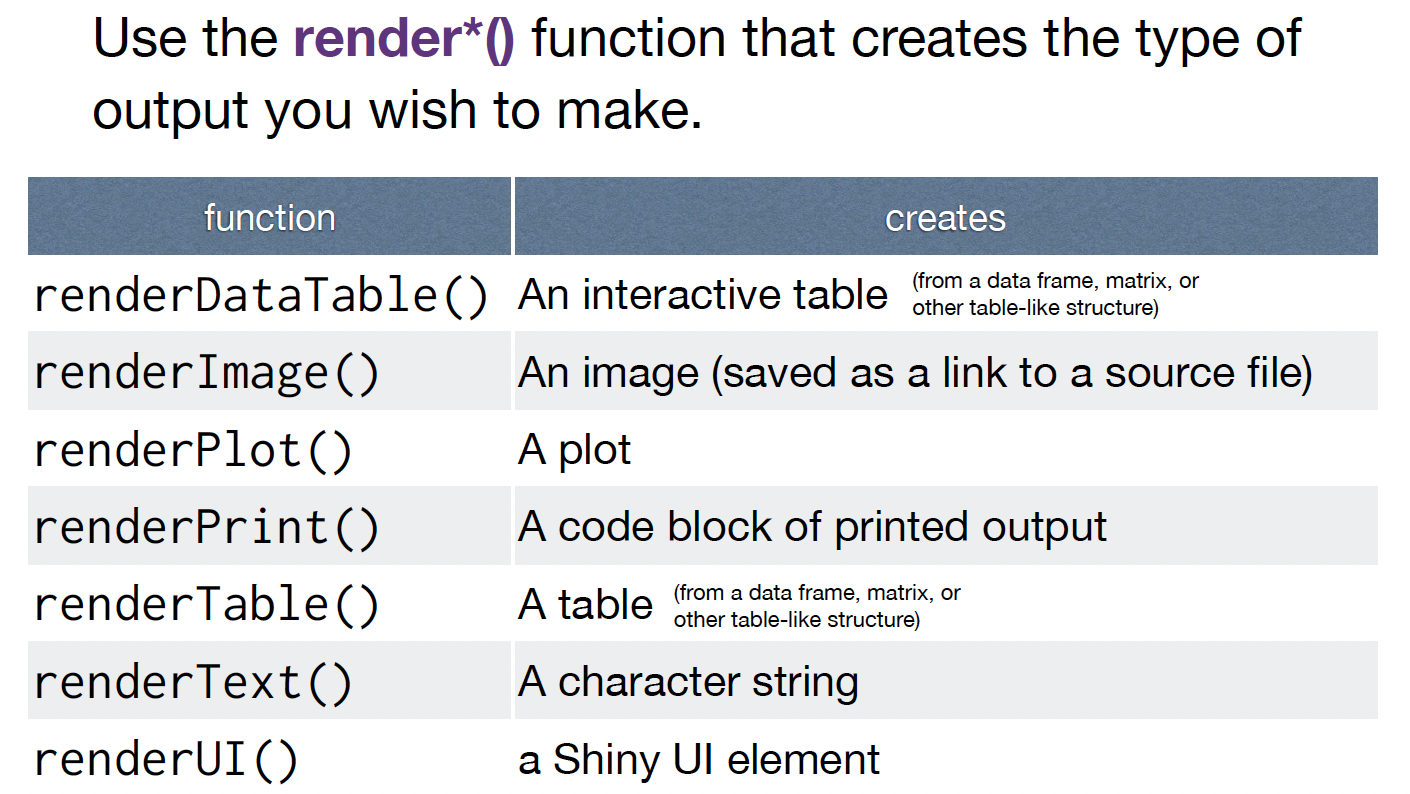
\includegraphics{shinyfigs/shiny_render3.png}
\end{frame}

\begin{frame}{Reactivity 101}
\phantomsection\label{reactivity-101}
The term \textbf{reactivity} refers to the idea that the inputs and
outputs are connected to each other: when you change and input, you
change all outputs that require the input.

Reactivity is an exciting charateristic, but can also get you in
trouble!
\end{frame}

\begin{frame}{Server recap}
\phantomsection\label{server-recap}
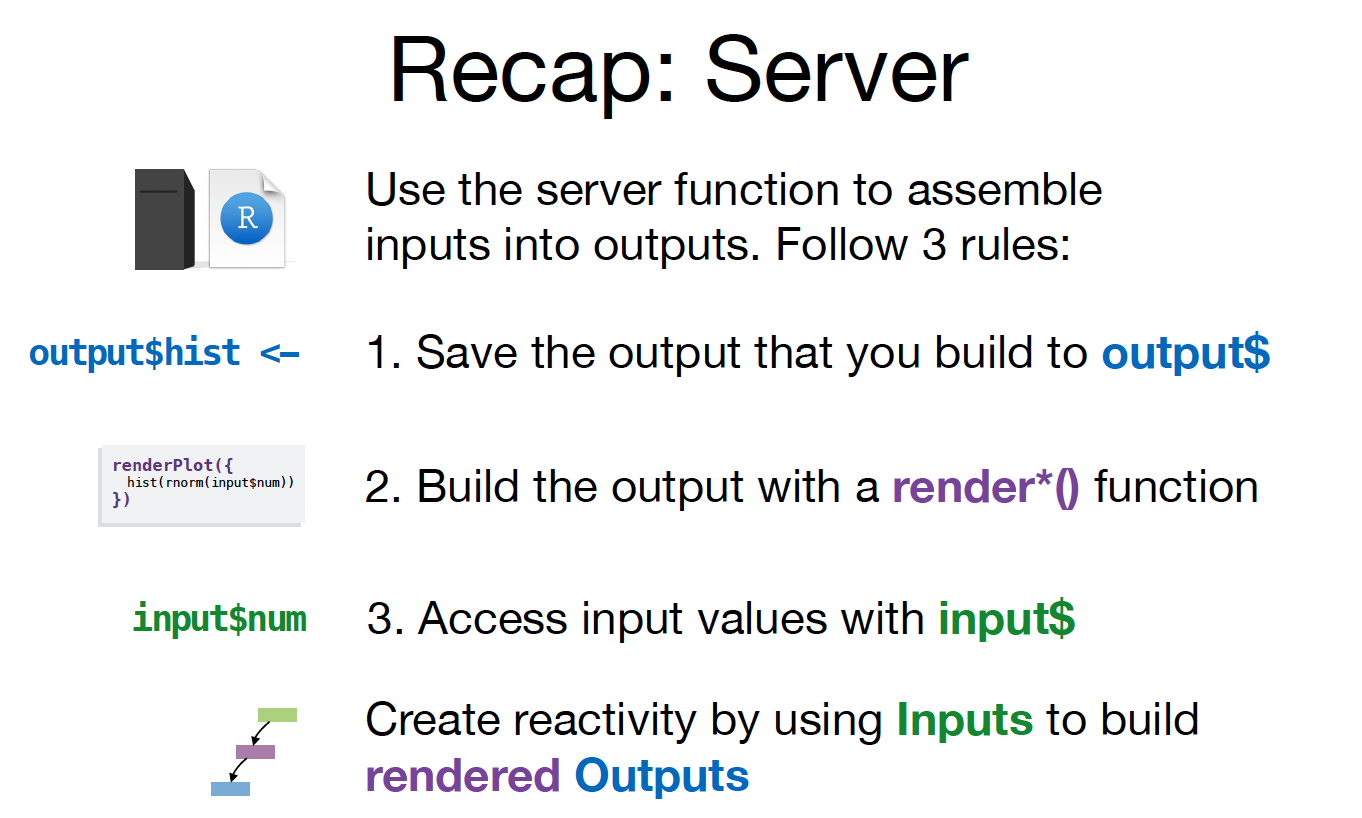
\includegraphics{shinyfigs/shiny_server_recap.png}
\end{frame}

\begin{frame}[fragile]{Complete Shiny app}
\phantomsection\label{complete-shiny-app}
Now putting everything together: \footnotesize

\begin{Shaded}
\begin{Highlighting}[]
\FunctionTok{library}\NormalTok{(shiny)}

\NormalTok{ui }\OtherTok{\textless{}{-}} \FunctionTok{fluidPage}\NormalTok{(}
  \FunctionTok{sliderInput}\NormalTok{(}\AttributeTok{inputId =} \StringTok{"num"}\NormalTok{,}
    \AttributeTok{label =} \StringTok{"Choose a number"}\NormalTok{,}
    \AttributeTok{value =} \DecValTok{25}\NormalTok{, }\AttributeTok{min =} \DecValTok{0}\NormalTok{, }\AttributeTok{max =} \DecValTok{100}\NormalTok{), }
  \FunctionTok{plotOutput}\NormalTok{(}\StringTok{"hist"}\NormalTok{)}
\NormalTok{  )}

\NormalTok{server }\OtherTok{\textless{}{-}} \ControlFlowTok{function}\NormalTok{(input, output)\{}
\NormalTok{  output}\SpecialCharTok{$}\NormalTok{hist }\OtherTok{\textless{}{-}} \FunctionTok{renderPlot}\NormalTok{(\{}
    \FunctionTok{hist}\NormalTok{(}\FunctionTok{rnorm}\NormalTok{(input}\SpecialCharTok{$}\NormalTok{num))}
\NormalTok{    \})}
\NormalTok{  \}}

\FunctionTok{shinyApp}\NormalTok{(}\AttributeTok{server =}\NormalTok{ server, }\AttributeTok{ui =}\NormalTok{ ui)}
\end{Highlighting}
\end{Shaded}
\end{frame}

\begin{frame}[fragile]{Multi-file apps:}
\phantomsection\label{multi-file-apps}
Now lets get more organized, create a \textbf{ui.R} file \footnotesize

\begin{Shaded}
\begin{Highlighting}[]
\CommentTok{\#ui.R}
\FunctionTok{library}\NormalTok{(shiny)}
\NormalTok{ui }\OtherTok{\textless{}{-}} \FunctionTok{fluidPage}\NormalTok{(}
  \FunctionTok{sliderInput}\NormalTok{(}\AttributeTok{inputId =} \StringTok{"num"}\NormalTok{,}
    \AttributeTok{label =} \StringTok{"Choose a number"}\NormalTok{,}
    \AttributeTok{value =} \DecValTok{25}\NormalTok{, }\AttributeTok{min =} \DecValTok{1}\NormalTok{, }\AttributeTok{max =} \DecValTok{100}\NormalTok{), }
  \FunctionTok{plotOutput}\NormalTok{(}\StringTok{"hist"}\NormalTok{)}
\NormalTok{  )}
\end{Highlighting}
\end{Shaded}

\normalsize

And a \textbf{server.R} file: \footnotesize

\begin{Shaded}
\begin{Highlighting}[]
\CommentTok{\#server.R}
\FunctionTok{library}\NormalTok{(shiny)}
\NormalTok{server }\OtherTok{\textless{}{-}} \ControlFlowTok{function}\NormalTok{(input, output)\{}
\NormalTok{  output}\SpecialCharTok{$}\NormalTok{hist }\OtherTok{\textless{}{-}} \FunctionTok{renderPlot}\NormalTok{(\{}
    \FunctionTok{hist}\NormalTok{(}\FunctionTok{rnorm}\NormalTok{(input}\SpecialCharTok{$}\NormalTok{num))}
\NormalTok{    \})}
\NormalTok{  \}}
\end{Highlighting}
\end{Shaded}
\end{frame}

\begin{frame}[fragile]{Multi-file apps:}
\phantomsection\label{multi-file-apps-1}
And then finally the program file, \textbf{app.R}:

\begin{Shaded}
\begin{Highlighting}[]
\CommentTok{\#app.R}
\FunctionTok{library}\NormalTok{(shiny)}

\FunctionTok{source}\NormalTok{(}\StringTok{"ui.R"}\NormalTok{)}
\FunctionTok{source}\NormalTok{(}\StringTok{"server.R"}\NormalTok{)}

\FunctionTok{shinyApp}\NormalTok{(}\AttributeTok{server =}\NormalTok{ server, }\AttributeTok{ui =}\NormalTok{ ui)}
\end{Highlighting}
\end{Shaded}
\end{frame}

\begin{frame}[fragile]{Building apps in R packages:}
\phantomsection\label{building-apps-in-r-packages}
In an R package, create an \texttt{inst/shiny} directory and place the
\texttt{Shiny} code there. Also:

\begin{itemize}
\tightlist
\item
  Write the package functions first!
\item
  This includes all analytics AND plotting functions
\item
  \texttt{Shiny} app should call functions, provide inputs, display
  results
\item
  Operate on high-quality R data objects!
\end{itemize}

Also, see examples from Dr.~Johnson's research, e.g.:
\url{https://github.com/compbiomed/animalcules}
\end{frame}

\begin{frame}[fragile]{Session Info}
\phantomsection\label{session-info}
\tiny

\begin{verbatim}
## R version 4.3.2 (2023-10-31)
## Platform: aarch64-apple-darwin20 (64-bit)
## Running under: macOS Ventura 13.5.1
## 
## Matrix products: default
## BLAS:   /Library/Frameworks/R.framework/Versions/4.3-arm64/Resources/lib/libRblas.0.dylib 
## LAPACK: /Library/Frameworks/R.framework/Versions/4.3-arm64/Resources/lib/libRlapack.dylib;  LAPACK version 3.11.0
## 
## locale:
## [1] en_US.UTF-8/en_US.UTF-8/en_US.UTF-8/C/en_US.UTF-8/en_US.UTF-8
## 
## time zone: America/Denver
## tzcode source: internal
## 
## attached base packages:
## [1] stats     graphics  grDevices utils     datasets  methods   base     
## 
## loaded via a namespace (and not attached):
##  [1] compiler_4.3.2    fastmap_1.1.1     cli_3.6.1         tools_4.3.2      
##  [5] htmltools_0.5.6.1 rstudioapi_0.15.0 yaml_2.3.7        rmarkdown_2.25   
##  [9] knitr_1.44        xfun_0.40         digest_0.6.33     rlang_1.1.1      
## [13] evaluate_0.22
\end{verbatim}
\end{frame}

\end{document}
